\documentclass[a4paper,12pt]{extarticle}
\usepackage[table,xcdraw]{xcolor}
\usepackage{pgfplots}
\usepackage[unicode, pdftex]{hyperref}
\usepackage[T2A]{fontenc}
\usepackage[utf8]{inputenc}
\usepackage[english,russian]{babel}
\usepackage{amsmath,amsfonts,amsthm, mathtools}
\usepackage{amssymb}
\usepackage{dsfont}
\usepackage{graphicx}
\graphicspath{{images/}}
\usepackage{wrapfig}
\usepackage{floatrow}
\usepackage{setspace}
\usepackage[headings]{fancyhdr}
\usepackage[margin=10pt,font={small,stretch=0,9},labelfont=bf,labelsep=period,
justification=centerlast]{caption}
\usepackage{array,tabularx,tabulary,booktabs}
\RequirePackage{multirow}
\RequirePackage{multicol}
\RequirePackage{longtable}
\usepackage{indentfirst}
\usepackage{hyperref}
\usepackage{icomma}
\newcommand*{\hm}[1]{#1\nobreak\discretionary{}
	{\hbox{$\mathsurround=0pt #1$}}{}}
\usepackage{soulutf8} 
\usepackage{etoolbox} 
\usepackage{geometry}
\geometry{top=20mm}
\geometry{bottom=20mm}
\geometry{left=20mm}
\geometry{right=20mm}
\DeclareMathOperator{\sgn}{\mathop{sgn}}
\usepackage[OT1]{fontenc}
\usepackage{amsmath}
\usepackage{amsfonts}
\usepackage{amssymb}
\usepackage{wasysym}
\usepackage{wrapfig}
\usepackage{physics}
\usepackage[normalem]{ulem}
\graphicspath{{pictures/}}
\DeclareGraphicsExtensions{.png,.jpg,.jpeg}
\usepackage{indentfirst}
\usepackage[T2A]{fontenc}
\usepackage{subfigure}
\usepackage{fancyhdr}
\usepackage{caption}

\usepackage{tabularx}
\usepackage{floatrow}
\usepackage{multicol}
\usepackage{lastpage}

\pgfplotsset{
  MyStyle1/.style={
    axis lines = middle,
    enlargelimits = true,
    grid=both,
    grid style={line width=.1pt, draw=gray!10},
    major grid style={line width=.2pt,draw=gray!50},
    minor tick num=5,
    enlargelimits=0.05,
    ticklabel style={font=\tiny,fill=white},
    xlabel style={at={(ticklabel* cs:1)},anchor=north west},
    ylabel style={at={(ticklabel* cs:1)},anchor=south east},
  }
}
\def\Slope{1.5}
\def\Intercept{-20}


% Настройка отчёркиваний и нумерации
\usepackage{fancyhdr}
\pagestyle{fancy}
\fancyhf{}

\fancyhead[L]{\nouppercase{\leftmark\hfill}}
\fancyfoot[RO, RE]{Страница \thepage \ из \pageref{LastPage}}
\renewcommand{\headrulewidth}{0.5pt}
\renewcommand{\footrulewidth}{0.5pt}

\usepackage{titlesec}
\titlelabel{\thetitle.\quad}

\pgfplotsset{compat=1.18}
\begin{document}

\thispagestyle{empty}
\begin{center}
	\textit{Федеральное государственное автономное образовательное\\ учреждение высшего образования }
	
	\vspace{0.5ex}
	
	\textbf{«Московский физико-технический институт\\ (национальный исследовательский университет)»}
\end{center}

\vspace{10ex}
\begin{figure}[!h]
  \begin{center}
    
\includegraphics[width = 0.8\textwidth]{MIPT.png}
  \end{center}
\end{figure}

\begin{center}
	
	\textbf{Лабораторная работа №5.1.3}
	
	\vspace{1ex}
	
	по курсу общей физики
	
	на тему:
	
	\textbf{\textit{<<Эффект Рамзауэра>>}}
	
	\vspace{20ex}
	
	\begin{flushright}
		\noindent
		\textit{Работу выполнил:}\\  
		\textit{Легких Никита \\(группа Б05-301)}
	\end{flushright}
	\vfill
	Долгопрудный \\ \today
	\setcounter{page}{1}
\end{center}
\newpage

% Конец шаблона
\newpage

\section*{Введение}
\textbf{Цель работы:} Исследовать энергетическую зависимость вероятности рассеяния электронов атомами инертного газа, определить энергии электронов при которых наблюдается <<просветление>> инертного газа и оценить размер его внешней электронной оболочки.

\section*{Теоретическая справка}

\begin{wrapfigure}{}{0.3\textwidth}
	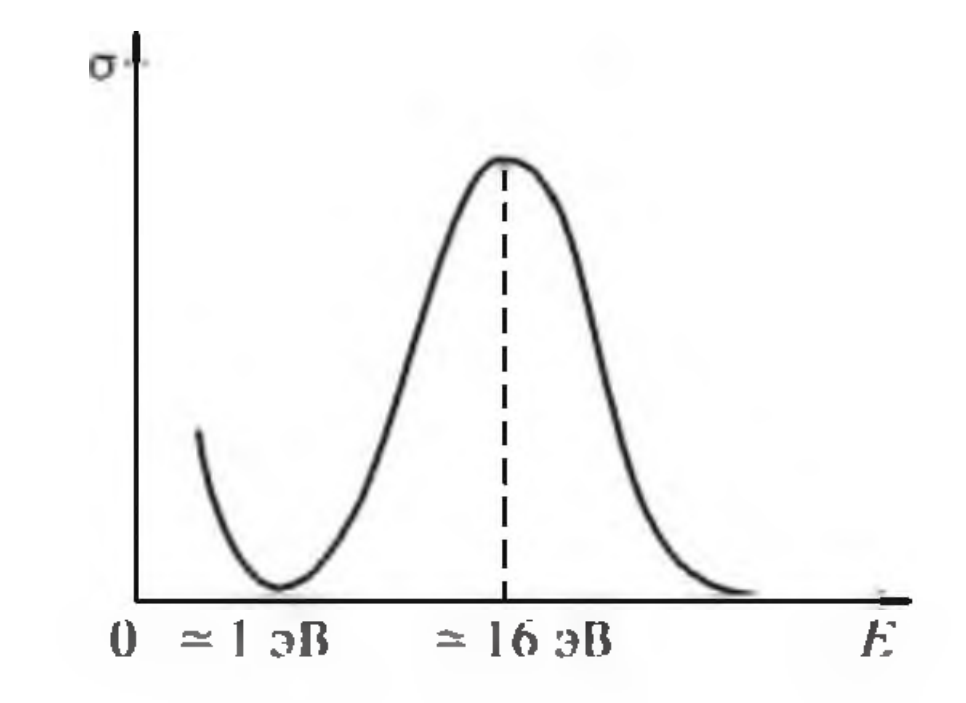
\includegraphics[width=1.0\linewidth]{pics/theor1.png}
	\caption{Качественная картина результатов измерения упругого рассеяния электронов в аргоне}
	\label{fig:screenshot1}
\end{wrapfigure}
Эффективное сечение реакции -- это величина, характеризующая вероятность перехода системы двух сталкивающихся частиц в результате их рассеяния (упругого или неупругого) в определенное конечное состояние. Сечение $ \sigma $ равно отношению числа $ N $ таких переходов в единицу времени к плотности потока рассеиваемых частиц $ n v $, падающих на мишень, т. е. к числу частиц, проходящих в единицу времени через единичную площадку, перпендикулярную к их скорости $ v $ ($ n $ -- плотность числа падающих частиц).
\begin{equation}\label{eq:sigma}
	\sigma = \frac{N}{n v}.
\end{equation}
Таким образом, сечение имеет размерность площади.


\begin{figure}[h]
	\centering
	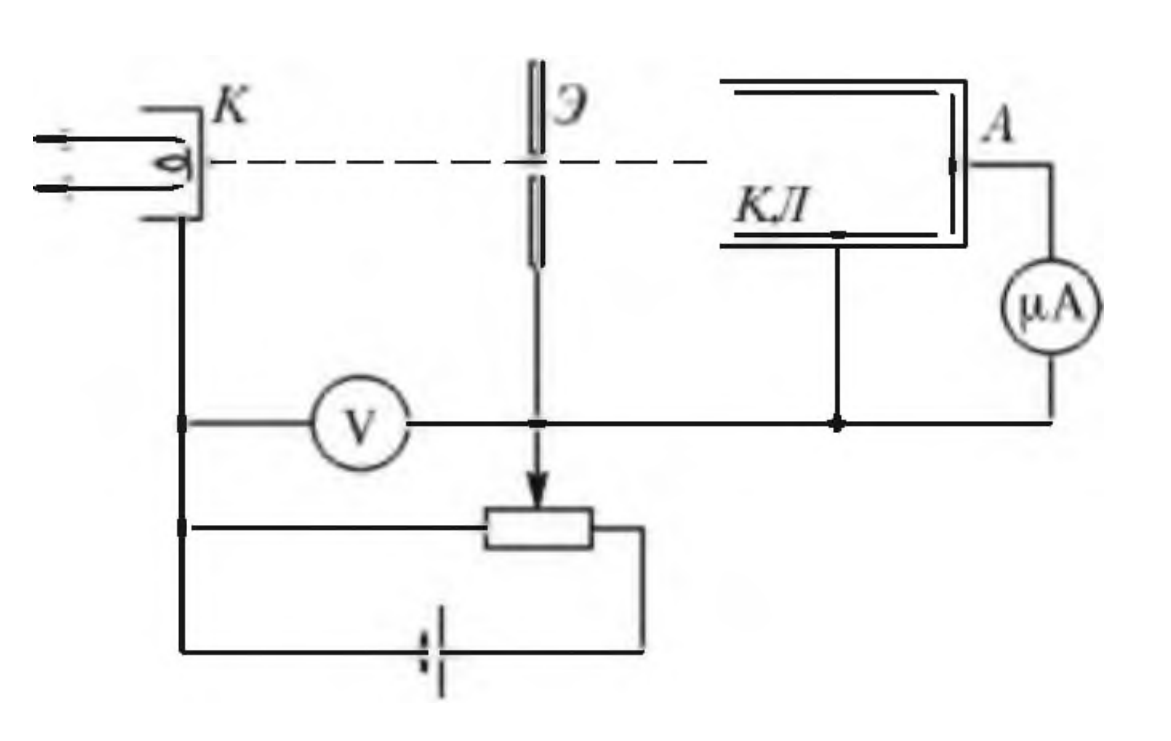
\includegraphics[width=0.5\linewidth]{pics/theor2}
	\caption{Схема установки для измерения сечения рассеяния электронов в газах}
\end{figure}
Качественно результат экспериментов Рамзауэра при энергии электронов порядка десятков эВ показан на рис. \ref{fig:screenshot1}.
По мере уменьшения энергии электрона от нескольких десятков электрон-вольт поперечное сечение его упругого рассеяния растет. Однако при энергиях меньше 16 эВ в случае аргона сечение начинает уменьшаться, а при $ E \sim 1 $ эВ практически равно нулю, т. е. аргон становится прозрачным для электронов. При дальнейшем уменьшении энергии электронов сечение рассеяния опять начинает возрастать. Это поведение поперечного сечения свойственно не только атомам аргона, но и атомам всех инертных газов. Такое поведение электронов нельзя объяснить с позиций классической физики. Объяснение этого эффекта потребовало учета волновой природы электронов. Схема эксперимента Рамзауэра показана, на рис. 1.


С точки зрения квантовой теории, внутри атома потенциальная энергия налетающего электрона $ U $ отлична от нуля, скорость электрона изменяется, становясь равной $ v' $ в соответствии с законом сохранения энергии
\begin{equation*}
	E = \frac{m v^2}{2} = \frac{m v'^2}{2}+ U,
\end{equation*}
а значит, изменяется и длина его волны де Бройля. Таким образом, по отношению к электронной волне атом ведет себя как преломляющая среда с относительным показателем преломления
\begin{equation*}
	n = \frac{\lambda}{\lambda'} = \sqrt{1-\frac{U}{E}}.
\end{equation*}

Коэффициент прохождения электронов максимален при условии
\begin{equation}\label{eq:at}
	\sqrt{\frac{2 m (E+U_0)}{\hbar^2}}l = \pi n;\; n \in \mathbb{N}_1,
\end{equation}
где $ U_0 $ -- глубина потенциальной ямы.

Это условие легко получить, рассматривая интерференцию электронных волн де Бройля в атоме. Движущемуся электрону соответствует волна де Бройля, длина которой определяется соотношением $ \lambda = h/m v $. Если кинетическая энергия электрона невелика, то $ E = m v^2/2 $ и $ \lambda = h/\sqrt{2 m E} $. При движении электрона через атом длина волны де Бройля становится меньше и равна $ \lambda' = h/\sqrt{2 m (E+U_0)} $ где $ U_0 $ — глубина атомного потенциала. При этом, волна де Бройля отражается от границ атомного потенциала, т. е. от поверхности атома, и происходит интерференция прошедшей через атом волны 1 и волны 2, отраженной от передней и задней границы атома (эти волны когерентны). Прошедшая волна 1 усилится волной 2, если геометрическая разность хода между ними $ \Delta = 2 l = \lambda' $, что соответствует условию первого интерференционного максимума, т. е. при условии
\begin{equation}\label{eq:condition}
	2 l = \frac{h}{\sqrt{2 m (E_1 + U_0)}}
\end{equation}
Прошедшая волна ослабится при условии
\begin{equation}\label{eq:condition2}
	2 l = \frac{3}{2}\frac{h}{\sqrt{2 m (E_1 + U_0)}}
\end{equation}

Из \eqref{eq:condition} и \eqref{eq:condition2}, можно получить
\begin{equation}\label{eq:radius}
	l = \frac{h \sqrt{5}}{\sqrt{32 m (E_2-E_1)}}.
\end{equation}
Оттуда же можно найти эффективную глубину потенциальной ямы атома:
\begin{equation}\label{eq:atomPit}
	U_0 = \frac{4}{5}E_2-\frac{9}{5} E_1.
\end{equation}

\subsection*{Расчётные формулы}

Уравнение вольт-амперной характеристики тиратрона:
\begin{equation}\label{eq:VAH}
	I_a = I_0 \cdot \exp(-C \omega (V));\; C = L n_a \Delta_a,
\end{equation}

где $ I_0 = e N_0 $ -- ток катода, а $ I_a = e N_a $ -- ток анода.
Отсюда определяется вероятность рассеяния электрона в зависимости от его энергии:
\begin{equation}\label{eq:probable}
	\omega (V) = -\frac{1}{C} \ln \frac{I_a(V)}{I_0}.
\end{equation}

\newpage
\section*{Экспериментальная установка}
\begin{figure}[h]
    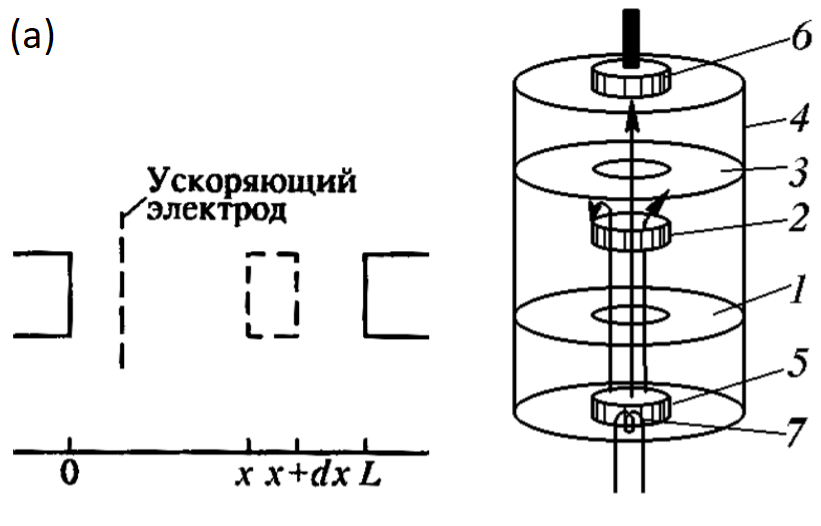
\includegraphics[width=0.42\textwidth]{pics/ustanovka1.png}
    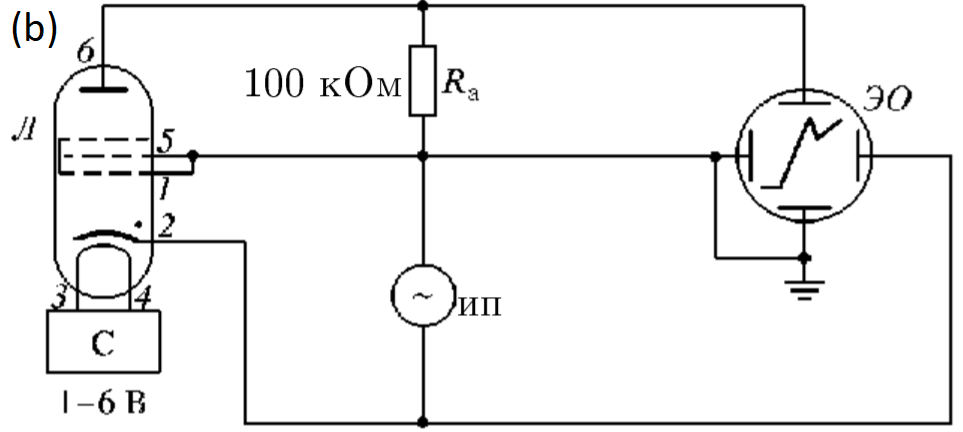
\includegraphics[width=0.57\textwidth]{pics/ustanovka2.png}
  \centering
  \caption{(a) Схема тиратрона (слева) и его конструкция (справа): 1,2,3 -- сетки, 4 -- внешний металлический цилиндр, 5 -- катод, 6 -- анод, 7 -- накаливаемая спираль. (b) Схема включения тиратрона.}
\end{figure}
Для изучения эффекта используется тиратрон ТГ3-01/1.3Б, заполненный инертным газом (Рис. 1а). Электроны эмитируются катодом, ускоряются напряжением $V$ и рассеиваются на атомах газа. Сетки соединены между собой и имеют один потенциал, примерно равный потенциалу анода. Рассеянные электроны отклоняются и уходят на сетку, а оставшиеся достигают анода, создавая ток $I_\text{a}$.
\begin{figure}[h]
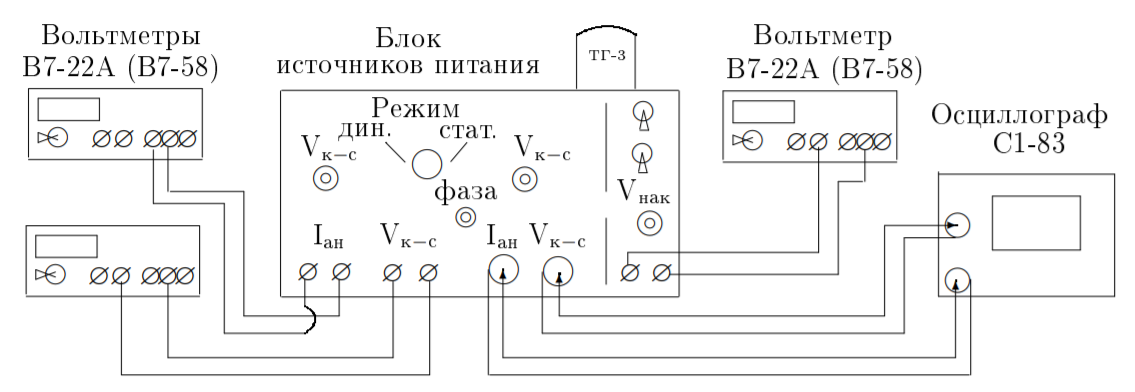
\includegraphics[width=0.9\textwidth]{pics/ustanovka3.png}
\centering
\caption{Схема установки.}
\end{figure}\\
Схема экспериментальной установки, изображенная на Рис. 1b, в нашей работе конструктивно осуществлена следующим образом (Рис. 2): лампа-тиратрон расположена непосредственно на корпусе блока источников питания (БИП), напряжение к электродам лампы подаётся от источников питания, находящихся в корпусе прибора. Регулировка напряжения и выбор режима работы установки производится при помощи ручек управления, выведенных на лицевую панель БИП.\\
В работе используются цифровые мультиметры модели GW Instek GDM-8145 и осциллограф модели GW Instek G0S-620.

\newpage
\section*{Ход работы}
\subsection*{Динамический режим}
Сначала проведем измерения в динамическом режиме осциллографа. 
\begin{table}[H]
    \centering
    \begin{tabular}{|c|c|c|c|}
        \hline
        $V_\text{накала}$, В & $V_{\text{max}}$, В & $V_{\text{min}}$, В & $V_\text{пробоя}$, В \\ \hline
        2,85 & 4 & 10 & 13 \\ \hline
        2,65 & 4 & 10 & 13 \\ \hline
        {$\sigma_\text{накала} = 0,01$ В} & \multicolumn{3}{c|}{{$\sigma_V = 1$ В}} \\ \hline
    \end{tabular}
    \caption{Результаты измерений}
\end{table}
Погрешность для накала берем как $\Delta V_{\text{накала}} = 0,0015 V_\text{накала}  + 0,003$ В, но, так как показания мультиметра немного менялись во времени (в пределах третьего знака после запятой), округлим ее до $0,01$ В. Погрешность же показаний, снятых с экрана осциллографа, будем считать равной одной цене деления (учтем погрешность установления "земли"), то есть $\sigma_V = 1$ В.\\ 
Ниже приведена фотография показаний осциллографа для $V_\text{накала} = 2.65$ В:
\begin{figure}[H]
    \centering
    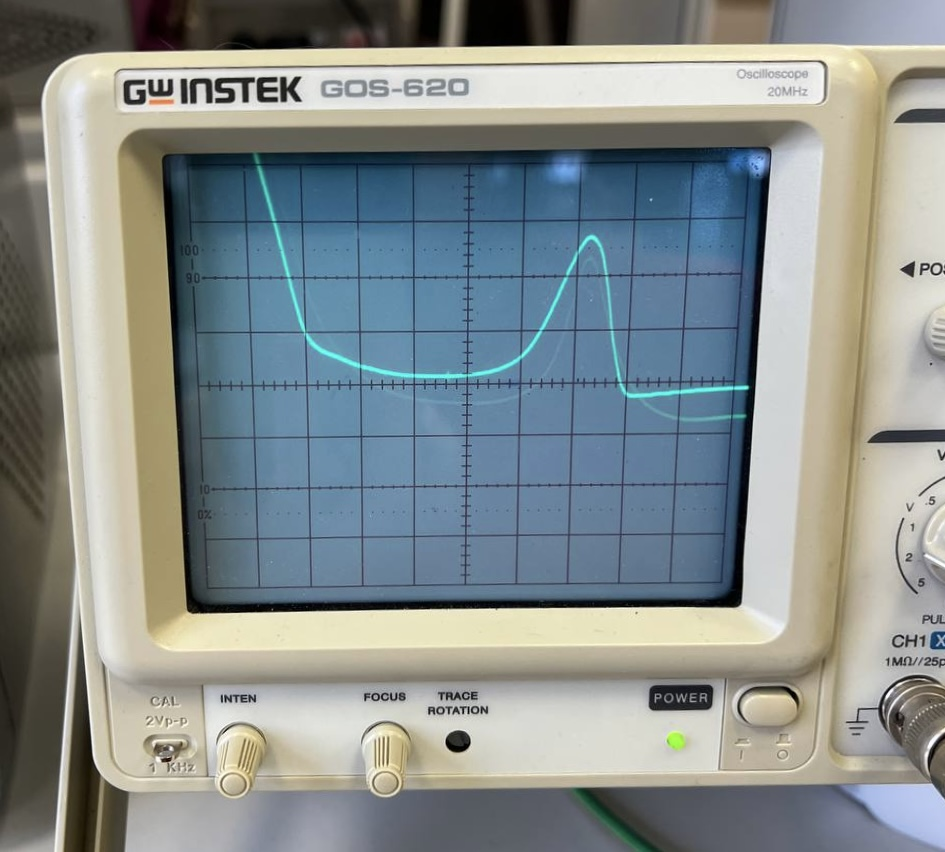
\includegraphics[width=0.45 \textwidth]{pics/1.jpeg}
\end{figure}
На основании приведенных выше измерений найдем размер электронной оболочки атома следующим формулам:
$$
l_1 = \dfrac{h}{2\sqrt{2m(E_1 + U_0)}}
\quad
l_2 = \dfrac{3}{4}\dfrac{h}{\sqrt{2m(E_2 + U_0)}}
\quad 
l_3 = \frac{h\sqrt{5}}{\sqrt{32m(E_2 - E_1)}}
$$
где $E_1 = eV_{\text{max}}$, $E_2 = eV_{\text{min}}$, $U_0 = 2,5$ эВ.\\
Погрешности вычисляются по формулам:
\begin{align*}
\sigma_{l_1} &= \sqrt{\left(\frac{\partial l_1}{\partial V_{\text{max}}}\right)^2 \sigma_{V_{\text{max}}}^2} = \sqrt{\left(\frac{h}{4\sqrt{2m(eV_{\text{max}}+U_0)^{3}}} \cdot e\right)^2 \sigma_{V_{\text{max}}}^2}
\end{align*}

\begin{align*}
\sigma_{l_2} &= \sqrt{\left(\frac{\partial l_2}{\partial V_{\text{min}}}\right)^2 \sigma_{V_{\text{min}}}^2} = \sqrt{\left(\frac{3h}{8\sqrt{2m(eV_{\text{min}}+U_0)^{3}}} \cdot e\right)^2 \sigma_{V_{\text{min}}}^2}
\end{align*}

\begin{gather*}
\sigma_{l_3} = \sqrt{\left(\frac{\partial l_3}{\partial V_{\text{max}}}\right)^2 \sigma_{V_{\text{max}}}^2 + \left(\frac{\partial l_3}{\partial V_{\text{min}}}\right)^2 \sigma_{V_{\text{min}}}^2} = \\
= \sqrt{\left(\frac{h\sqrt{5}}{2\sqrt{32m(E_2-E_1)^3}} \cdot e\right)^2 \sigma_{V_{\text{max}}}^2 + \left(\frac{h\sqrt{5}}{2\sqrt{32m(E_2-E_1)^3}} \cdot e\right)^2 \sigma_{V_{\text{min}}}^2}
\end{gather*}

Также оценим глубину потенциальной ямы по формуле:
$$
U_0 = \frac{4}{5}E_2 - \frac{9}{5}E_1
$$
Погрешность вычисляется как:
\begin{align*}
\sigma_{U_0} &= \sqrt{\left(\frac{\partial U_0}{\partial V_{\text{max}}}\right)^2 \sigma_{V_{\text{max}}}^2 + \left(\frac{\partial U_0}{\partial V_{\text{min}}}\right)^2 \sigma_{V_{\text{min}}}^2} = \\
&= \sqrt{\left(-\frac{9}{5}e\right)^2 \sigma_{V_{\text{max}}}^2 + \left(\frac{4}{5}e\right)^2 \sigma_{V_{\text{min}}}^2}
\end{align*}

Результаты внесем в таблицу ниже:
\begin{table}[H]
\centering
{\begin{tabular}{|c|c|c|c|c|}
\hline
$V_\text{накала}$, В & $l_1$, \AA & $l_2$, \AA & $l_3$, \AA & $U_0$, эВ \\ \hline
2.85 & $2,24 \pm 0,15$ & $2,60 \pm 0,10$ & $3,1 \pm 0,6$ & $-1,0 \pm 2,6$ \\ \hline
2,64 & $2,41 \pm 0,19$ & $2,60 \pm 0,10$ & $2,80 \pm 0,47$ & $0,8 \pm 2,6$ \\ \hline
\end{tabular}}
\caption{Обработка данных}
\end{table}
Везде в ходе работы мы считаем погрешность как погрешность сложной функции, то есть через корень суммы частных производных на относительную погрешность в квадрате.\\
Заметим, что значения $l$, посчитанные по разным формулам, хоть и имеют общий порядок величины, но все же не совпадают в пределах доверительных интервалом, что, вероятно, может быть связано с тем, что реальная глубина ямы на самом деле намного меньше, чем принятая для расчетов - это видно из посчитанных для нее значений. При этом у всех полученных результатов достаточно большая погрешность, связанная с погрешностью изначальных измерений. Таким образом, этот способ подходит скорее для оценки порядка величины, чем для точных вычислений.\\
Далее оценим ионизационный потенциал инертного газа:
\[U_1 = U_0 + V_{\text{пробоя}} = (12,0 \pm 3,6) \text{ В}\]
\[U_2 = U_0 + V_{\text{пробоя}} = (13,8 \pm 3,6) \text{ В}\]
Погрешность вычисляется по формуле:
\[
\sigma_{U_i} = \sqrt{\sigma_{U_0}^2 + \sigma_{V_{\text{пробоя}}}^2}
\]
Таким образом, сравнив полученные значения с табличными, можем сделать вывод, что в данной работе мы скорее всего имеем дело с ксеноном.

\newpage

\subsection*{Статический режим}
Снимем ВАХ тиратрона, результаты внесем в таблицу ниже:	

Далее считается что $V_1 = V_{\text{катод-сетка}},$ $V_2 = V_{\text{анод}}$.
\begin{table}[H]
\centering
\small
\begin{tabular}{|c|c|c|c|c|c|c|c|}
\hline
\multicolumn{4}{|c|}{$V_{\text{накала}} = 2.85$ В} & \multicolumn{4}{|c|}{$V_{\text{накала}} = 2,94$ В} \\ \hline
$V_1$, В& $V_2$, В& $\sigma_{V_1}$, В& $\sigma_{V_2}$, В& $V_1$, В& $V_2$, В& $\sigma_{V_1}$, В& $\sigma_{V_2}$, В\\ \hline
0.17& 0.0& 0.00& 0.0& 11.5& 42.9& 0.06& 0.2\\ \hline
2.07& 0.1& 0.01& 0.0& 11.0& 41.6& 0.06& 0.2\\ \hline
2.17& 0.4& 0.01& 0.0& 10.5& 40.6& 0.06& 0.2\\ \hline
2.27& 0.8& 0.01& 0.0& 10.3& 39.7& 0.05& 0.2\\ \hline
2.32& 1.1& 0.01& 0.0& 10.1& 39.6& 0.05& 0.2\\ \hline
2.35& 2.8& 0.01& 0.0& 9.9& 39.7& 0.05& 0.2\\ \hline
2.43& 4.6& 0.01& 0.0& 9.6& 40.7& 0.05& 0.2\\ \hline
2.48& 5.8& 0.01& 0.0& 9.4& 41.5& 0.05& 0.2\\ \hline
2.51& 10.3& 0.01& 0.1& 9.2& 42.1& 0.05& 0.2\\ \hline
2.65& 12.4& 0.01& 0.1& 8.9& 43.5& 0.05& 0.2\\ \hline
3.12& 43.5& 0.02& 0.2& 8.4& 47.6& 0.04& 0.3\\ \hline
3.35& 51.7& 0.02& 0.3& 7.9& 52.4& 0.04& 0.3\\ \hline
3.53& 54.8& 0.02& 0.3& 7.2& 58.8& 0.04& 0.3\\ \hline
3.76& 54.3& 0.02& 0.3& 6.9& 62.2& 0.04& 0.3\\ \hline
4.02& 57.4& 0.02& 0.3& 6.6& 64.9& 0.03& 0.3\\ \hline
4.25& 59.3& 0.02& 0.3& 6.0& 67.7& 0.03& 0.4\\ \hline
4.51& 60.5& 0.02& 0.3& 5.5& 68.9& 0.03& 0.4\\ \hline
4.79& 61.1& 0.03& 0.3& 5.3& 69.1& 0.03& 0.4\\ \hline
5.03& 61.0& 0.03& 0.3& 5.1& 69.0& 0.03& 0.4\\ \hline
5.27& 60.4& 0.03& 0.3& 4.8& 68.7& 0.03& 0.4\\ \hline
       5.55&          59.1&         0.03&         0.3& 4.5& 67.3& 0.02& 0.4\\ \hline
       5.91&          57.2&         0.03&         0.3& 4.1& 64.6& 0.02& 0.3\\ \hline
       6.22&          55.2&         0.03&         0.3& 3.5& 56.9& 0.02& 0.3\\ \hline
       6.53&          52.7&         0.03&         0.3& 3.2& 50.0& 0.02& 0.3\\ \hline
       6.78&          50.4&         0.04&         0.3& 2.9& 32.7& 0.02& 0.2\\ \hline
       7.10&          47.1&         0.04&         0.2& 2.5& 7.1& 0.01& 0.0\\ \hline
       7.53&          42.8&         0.04&         0.2& 2.0& 0.0& 0.01& 0.0\\ \hline
       7.90&          39.6&         0.04&         0.2& & & & \\ \hline
       8.27&          36.4&         0.04&         0.2& & & & \\ \hline
       8.56&          34.4&         0.05&         0.2& & & & \\ \hline
 8.98& 31.8& 0.05& 0.2& & & &\\\hline
 9.77& 29.1& 0.05& 0.2& & & &\\\hline
 10.44& 30.4& 0.06& 0.2& & & &\\\hline
 10.60& 30.5& 0.06& 0.2& & & &\\\hline
 10.83& 30.6& 0.06& 0.2& & & &\\\hline
 11.08& 31.1& 0.06& 0.2& & & &\\\hline
 11.62& 32.3& 0.06& 0.2& & & &\\ \hline
\end{tabular}
\caption{Результаты измерений}
\end{table}
Показания тока анода можно получить, поделив значения $V_I$ на сопротивление $R = 100$ кОм.\\
На основании полученных результатов построим график ВАХ:

\begin{minipage}{1\textwidth}
    \begin{tikzpicture}
        \begin{axis}[
            width=0.8\textwidth,
            height=,
            xlabel={$V_{\text{катод}}$, В},
            ylabel={$V_{\text{анод}}$, В},
            MyStyle1,
            legend pos=north west, % Положение легенды
            legend cell align=left, % Выравнивание текста легенды
            legend style={font=\small}, % Стиль легенды
        ]
            % Первый график
            \addplot [
                only marks,
                mark=*, % Маркер
                color=black, % Цвет (если не указан в MyStyle1)
                error bars/.cd,
                    x dir=both,
                    x explicit,
                    y dir=both,
                    y explicit,
            ] table [
                x=v1,
                y=v2,
                x error minus=sigmav1,
                x error plus=sigmav1,
                y error minus=sigmav2,
                y error plus=sigmav2,
                col sep=comma
            ] {tables/2.65.csv};
            \addlegendentry{Данные 2.65 В} % Текст для первого графика
            
            % Второй график
            \addplot [
                purple,
                only marks,
                mark=square*, % Другой маркер для различия
                error bars/.cd,
                    x dir=both,
                    x explicit,
                    y dir=both,
                    y explicit,
            ] table [
                x=v1,
                y=v2,
                x error minus=sigmav1,
                x error plus=sigmav1,
                y error minus=sigmav2,
                y error plus=sigmav2,
                col sep=comma
            ] {tables/2.94.csv};
            \addlegendentry{Данные 2.94 В} % Текст для второго графика
        \end{axis}
    \end{tikzpicture}
\end{minipage}

Из графиков получим:
\begin{table}[H]
    \centering
    \begin{tabular}{|c|c|c|}
        \hline
        $V_\text{накала}$, В & $V_{\text{max}}$, В & $V_{\text{min}}$, В \\ \hline
        2.95 & $5,2 \pm 0,1$ & $10.1 \pm 0,1$ \\ \hline
        2,65 & $4,9 \pm 0,1$ & $10.0 \pm 0,4$ \\ \hline
    \end{tabular}
    \caption{Анализ графиков}
\end{table}
На основании этих данных, проведем аналогичные расчеты:
\begin{table}[H]
\centering
{\begin{tabular}{|c|c|c|c|c|}
\hline
$V_\text{накала}$, В & $l_1$, \AA & $l_2$, \AA & $l_3$, \AA & $U_0$, эВ \\ \hline
2.94 & $2.21 \pm 0.04$ & $2.62 \pm 0.03$ & $3.10 \pm 0,4$ & $-1.3 \pm 0.5$ \\ \hline
2,65 & $2.26 \pm 0.05$ & $2.58 \pm 0.06$ & $3.06 \pm 0.6$ & $-0.8 \pm 0.7$ \\ \hline
\end{tabular}}
\caption{Обработка данных}
\end{table}
Используя формулу для интерференционных максимумов:
\[
k_2 l = \sqrt{\frac{2m(E_n + U_0)}{\hbar^2}} \, l = n\pi, \quad n = 1, 2, 3, 4, \dots
\]
выразим энергию электрона:
\[
E_n = \frac{n^2\pi^2\hbar^2}{2ml^2} - U_0 = n^2(E_1 + U_0) - U_0.
\]
Погрешность вычисляется по формуле:
\[
\sigma_{E_n} = \sqrt{\left(\frac{\partial E_n}{\partial E_1}\right)^2 \sigma_{E_1}^2 + \left(\frac{\partial E_n}{\partial U_0}\right)^2 \sigma_{U_0}^2}
= \sqrt{(n^2)^2 \sigma_{E_1}^2 + (n^2 - 1)^2 \sigma_{U_0}^2}
\]
По полученной формуле оценим значения напряжений максимумов порядка $n > 2$:
\begin{table}[H]
\centering
\begin{tabular}{|c|c|c|c|}
\hline
$V_{\text{накала}}$, В & $E_2$, эВ & $E_3$, эВ & $E_4$, эВ \\ \hline
2.94 & & $21.2 \pm 10.1$ & $35.2 \pm 11.7$ \\ \hline
2,65 & $22.0 \pm 7.3$ & $50.5 \pm 10.5$ & $90.4 \pm 12.1$ \\ \hline
\end{tabular}
\end{table}
Полученные энергии выше потенциала ионизации, поэтому эти максимумы уже не будут наблюдаться.
На основании формулы 
\begin{equation}
w(V) = -\frac{1}{C} \ln \frac{I_a(V)}{I_0}
\end{equation}
Построим график $w(V)$ (а точнее график $-\ln I(V)$ - равный $w(V)$ с точностью домножения и прибавления константы):

\begin{minipage}{1\textwidth}
    \begin{tikzpicture}
        \begin{axis}[
            width=0.8\textwidth,
            height=,
            xlabel={$V$, В},
            ylabel={$-\ln(I)$, В},
            MyStyle1, 
            legend pos=north west, % Положение легенды
            legend cell align=left, % Выравнивание текста легенды
            legend style={font=\small}, % Стиль легенды
        ]
            % Первый график
            \addplot [
                only marks,
                mark=*, % Маркер
                color=black, % Цвет (если не указан в MyStyle1)
            ] table [
                x=v,
                y=lnV,
                col sep=comma
            ] {tables/lnI.csv};
            \addlegendentry{$w(V)$ с точностью до коефициента и смещения} % Текст для первого графика
        \end{axis}
    \end{tikzpicture}
\end{minipage}

\section*{Выводы}
В ходе лабораторной работы удалось:
\begin{itemize}
\item исследовать энергетическую зависимость вероятности рассеяния электронов атомами инертного газа и получить график $w(V)$ для двух значений $V_{\text{накала}}$,
\item определить энергии электронов, при которых наблюдается <<просветление>> инертного газа:
\begin{itemize}
\item для $V_{\text{накала}} = 2,95$ В: $V_{\text{max}} = (5,2 \pm 0,1)$ В, $V_{\text{min}} = (10,1 \pm 0,1)$ В
\item для $V_{\text{накала}} = 2,65$ В: $V_{\text{max}} = (4,9 \pm 0,1)$ В, $V_{\text{min}} = (10,0 \pm 0,4)$ В
\end{itemize}
\item оценить размер внешней электронной оболочки инертного газа:
\begin{itemize}
\item по данным динамического режима: $l = (2,59 \pm 0,27)$ \AA
\item по данным статического режима: $l = (2,69 \pm 0,17)$ \AA
\end{itemize}
\item определить, что исследуемый газ, вероятно, является ксеноном, так как полученный ионизационный потенциал $U = (12,9 \pm 3,6)$ В близок к табличному значению 12,13 В для ксенона
\i
\end{itemize}



% \section*{Выводы}
% В ходе лабораторной работы удалось:
% \begin{itemize}
%     \item исследовать энергетическую зависимость вероятности рассеяния электронов атомами инертного газа и получить график $w(V)$ для двух значений $V_{\text{накала}}$, 
%     \item определить энергии электронов при которых наблюдается <<просветление>> инертного газа  
%     \item оценить размер внешней электронной оболочки инертного газа, среднее значение по вычислениям в динамическом режиме - $l = (2,59 \pm 0,27)$ \AA, в статическом - $l = (2,69 \pm 0,17)$ \AA, оба результата в пределах доверительных интервалов совпадают с табличным значением $2,8$ \AA.
% \end{itemize}
\end{document}